\documentclass[conference]{IEEEtran}
\IEEEoverridecommandlockouts

\usepackage{cite}
\usepackage{amsmath,amssymb,amsfonts}
\usepackage{graphicx}
\usepackage{booktabs}
\usepackage{url}
\usepackage{xcolor}

\begin{document}

\title{Information Richness Ablation for Multimodal Land Cover Composition Regression: A Leakage-Free Study\\
{\large Phase 2 Report --- Transformers Course Project (DRAFT)}}

\author{\IEEEauthorblockN{\"Omer Faruk Merey}
\IEEEauthorblockA{Middle East Technical University \\
omer.merey@metu.edu.tr}}

\maketitle

\begin{abstract}
We study whether auxiliary textual captions improve land cover composition
regression from satellite imagery, under strict no-leakage conditions. Phase 1
exposed that hybrid and text-only captions in the ARAS400k dataset embed the
ground-truth percentages verbatim, rendering the regression task trivially
solvable from text. Phase 2 reformulates the task as an
\emph{Information Richness} ablation across four levels of textual
guidance --- a vision-only baseline (two architectural variants), a
keyword-list condition derived from vision-only captions, and a qualitative
condition consisting of fully sanitized vision-only captions evaluated for
both Gemma-3 and Qwen-3-VL caption sources. CLIP ViT-B/32 encoders are kept
frozen; only a cross-attention fusion module and a small MLP regression head
are trained, across 5 conditions $\times$ 3 seeds. Empirically, additional
clean text does \emph{not} reduce test MSE relative to an empty-caption
baseline that shares the same fusion architecture, while a pure-vision
architecture without cross-attention performs noticeably worse than all
caption-bearing conditions. We argue this dissociates two effects that the
original Phase 1 plan would have conflated: (i) the architectural contribution
of the cross-attention layer, and (ii) the semantic contribution of the text.
The findings also offer indirect support for the leakage hypothesis: when
percentages are stripped, the residual qualitative content carries no useful
multimodal signal beyond the vision encoder itself.
\end{abstract}

\begin{IEEEkeywords}
remote sensing, land cover, multimodal learning, CLIP, cross-attention, data
leakage, ablation
\end{IEEEkeywords}

%-------------------------------------------------------------------------
\section{Introduction}

Land cover composition is a structured regression target with seven mutually
exclusive classes (Tree, Shrub, Grass, Crop, Built-up, Barren, Water) summing
to 100\,\%. The ARAS400k dataset~\cite{aras400k} provides matched RGB tiles,
pixel-level masks, and five caption variants generated by vision-language and
text-only models.

Phase 1 introduced a CLIP-based vision-text architecture with multi-head
cross-attention fusion. Feedback from the course instructor flagged a
structural \textbf{data leakage} problem: the \texttt{hybrid\_*} and
\texttt{text\_qwen3-4b} caption variants explicitly contain the GT percentages
(e.g.\ ``grasslands (92\,\%)''). Even a sanitization pass that strips the
digits is insufficient, because the very vision-language models that produced
those captions saw the ground-truth percentages and shaped the qualitative
narrative around them; the leakage is structural, not lexical.

We restructure the study around an \textbf{Information Richness} ablation.
The new research question is:

\begin{quote}
\emph{How does the semantic richness of auxiliary text captions --- ranging
from a vision-only baseline, to simple keywords, to detailed qualitative
descriptions --- impact the accuracy of land cover composition regression
from satellite images while strictly avoiding data leakage?}
\end{quote}

\textbf{Contributions.}
(1)~A leakage-free five-condition ablation that decomposes textual contribution
into low-richness (keyword sets) and high-richness (sanitized full captions).
(2)~An architectural control (R0b) that isolates the cross-attention layer's
contribution from any text contribution.
(3)~An empirical finding that no level of clean vision-only text significantly
improves over an empty-caption baseline that shares the same fusion
architecture, while the architectural control underperforms all
caption-bearing variants.

%-------------------------------------------------------------------------
\section{Methodology}

\subsection{Data Leakage Mitigation and Text Sanitization}

The central challenge identified in Phase 1 was the presence of ground-truth
percentages within the textual descriptions (e.g.\ ``92\,\% grass''), which
rendered the regression task trivial. We address this on two layers:

\paragraph{Source isolation} The model exclusively uses
\texttt{vision\_gemma3-4b} and \texttt{vision\_qwen3-vl-8b} captions. Unlike
the \texttt{hybrid\_*} variants, these were generated by VLM models that saw
only the image, so they are inherently free from ground-truth knowledge ---
i.e., free from the structural (indirect) leakage that ``hybrid'' captions
carry through narrative shaping.

\paragraph{Sanitization pipeline} A regex-based safety filter
\verb|\b\d+(?:\.\d+)?%?| replaces every integer, decimal, and percentage
token with the placeholder \texttt{[NUM]}. Vision-only captions are nominally
number-free, so this functions as a defense against hallucinated digits and
preserves the project's commitment to explicit sanitization. The result is a
purely qualitative semantic cue (e.g.\ ``extensive grasslands'' instead of
``92\,\% grass'').

\subsection{Information Richness Levels}

The study evaluates the model across four levels of semantic guidance
(Table~\ref{tab:conditions}).

\begin{table}[ht]
\centering
\caption{Five experimental conditions (5 $\times$ 3 seeds = 15 runs).
``CA'' is multi-head cross-attention; ``GAP'' is patch-token mean pooling.}
\label{tab:conditions}
\begin{tabular}{@{}lll@{}}
\toprule
\textbf{Code} & \textbf{Architecture} & \textbf{Text input} \\
\midrule
R0a & CLIP+CA+MLP & \texttt{""} (empty token) \\
R0b & CLIP+GAP+MLP & --- (no text path) \\
R1  & CLIP+CA+MLP & noun-lemma NER over both \texttt{vision\_*} \\
R2a & CLIP+CA+MLP & sanitized \texttt{vision\_gemma3-4b} \\
R2b & CLIP+CA+MLP & sanitized \texttt{vision\_qwen3-vl-8b} \\
\bottomrule
\end{tabular}
\end{table}

\begin{itemize}
\item \textbf{R0 (dual baselines).}
  \emph{R0a} keeps the full multimodal architecture but feeds an empty caption,
  isolating the impact of textual content while holding model capacity
  constant.
  \emph{R0b} removes cross-attention entirely (pure ViT $\rightarrow$ GAP
  $\rightarrow$ MLP), serving as the fundamental performance floor.
\item \textbf{R1 (keyword level).} Input is a comma-separated lemma list
  obtained by running spaCy \texttt{en\_core\_web\_sm} over the sanitized
  concatenation of both \texttt{vision\_*} captions and taking the lemmatized
  head of every noun chunk (\texttt{isalpha}, length $> 2$). We deliberately
  do \emph{not} restrict the lemma vocabulary to the seven target classes:
  any such filter would require a hand-built map from observed nouns to
  target classes, which would inject GT structure into the input. The model
  learns the mapping from data.
\item \textbf{R2 (qualitative level), with dual comparison.}
  R2a uses sanitized \texttt{vision\_gemma3-4b} captions; R2b uses sanitized
  \texttt{vision\_qwen3-vl-8b}. Training both lets us benchmark which
  vision-LLM provides better semantic alignment for this remote-sensing task.
\end{itemize}

\subsection{Architecture and Training Strategy}

\paragraph{Encoder freezing} Both CLIP ViT-B/32 image and CLIP text encoders
are kept frozen during training. This ensures any performance gains are
attributable to the cross-attention fusion layer and the semantic richness of
the input, not to the encoders adapting to the remote-sensing domain. Only
the cross-attention block ($\sim$1.05\,M parameters) and the
\texttt{Linear}(512$\rightarrow$256)$\rightarrow$\texttt{ReLU}$\rightarrow$\texttt{Linear}(256$\rightarrow$7)$\rightarrow$\texttt{Softmax}
head ($\sim$0.13\,M parameters) are trained.

\paragraph{Fusion} The fusion block uses a single multi-head cross-attention
layer (\texttt{embed\_dim}=512, 8 heads), with image patches as queries and
text tokens as keys/values:
\(
\mathrm{Fused} = \mathrm{MHA}(Q = P_\text{img}, K = T_\text{txt}, V = T_\text{txt}).
\)
The 49 fused vectors are mean-pooled before the MLP head. For R0b the
cross-attention block is removed and pooled patch features go directly into
the head.

\paragraph{Optimization} AdamW (lr $= 10^{-4}$, weight decay $10^{-4}$),
cosine annealing over 30 epochs, batch size 128, early stopping with patience
5 on validation MSE. Loss is mean squared error between predicted and target
distributions, both normalized to sum to 1.

\paragraph{Compute and reproducibility} Because CLIP encoders are frozen,
their forward pass is identical at every epoch. We exploit this by
precomputing image patch embeddings ($N \times 49 \times 512$, fp16) and
per-condition text token embeddings ($N \times 77 \times 512$, fp16) once,
storing them on disk, and consuming them directly inside the training loop.
This is mathematically equivalent to running CLIP per batch but reduces the
full 5$\times$3 grid wall-clock from approximately 10 hours of online
training on an Apple M4 MacBook Pro to under 40 minutes including
precomputation. All runs are tracked via Weights \& Biases for full
reproducibility, with run names of the form
\texttt{\{condition\}\_seed\{seed\}}.

\subsection{Dataset and Splits}

ARAS400k contains 10\,000 RGB tiles ($256 \times 256$) with seven-class
composition percentages and the five caption variants. All samples carry the
\texttt{synth} split tag; we re-split deterministically 70/15/15 (train/val/test,
seed 42) without modifying the source CSV.

%-------------------------------------------------------------------------
\section{Results}

\subsection{Main Metrics}

Table~\ref{tab:mse} reports test set metrics aggregated across the three
seeds. Fig.~\ref{fig:bar} visualizes mean test MSE with one-standard-deviation
error bars.

\begin{table}[ht]
\centering
\caption{Test set metrics, mean $\pm$ std over 3 seeds.
Lower is better for all metrics.}
\label{tab:mse}
\begin{tabular}{@{}lcccc@{}}
\toprule
\textbf{Cond.} & \textbf{MSE} $\downarrow$ & \textbf{MAE} $\downarrow$
& \textbf{RMSE} $\downarrow$ & \textbf{KL} $\downarrow$ \\
\midrule
R0a & \textbf{0.00707}$\pm$0.00006 & \textbf{0.0406}$\pm$0.0003 & 0.0841$\pm$0.0003 & 0.140$\pm$0.002 \\
R0b & 0.01101$\pm$0.00032 & 0.0554$\pm$0.0011 & 0.1049$\pm$0.0015 & 0.226$\pm$0.006 \\
R1  & 0.00760$\pm$0.00016 & 0.0425$\pm$0.0008 & 0.0872$\pm$0.0009 & 0.152$\pm$0.003 \\
R2a & 0.00751$\pm$0.00026 & 0.0422$\pm$0.0009 & 0.0867$\pm$0.0014 & 0.149$\pm$0.006 \\
R2b & 0.00739$\pm$0.00020 & 0.0421$\pm$0.0007 & 0.0859$\pm$0.0010 & 0.148$\pm$0.003 \\
\bottomrule
\end{tabular}
\end{table}

\begin{figure}[ht]
\centering
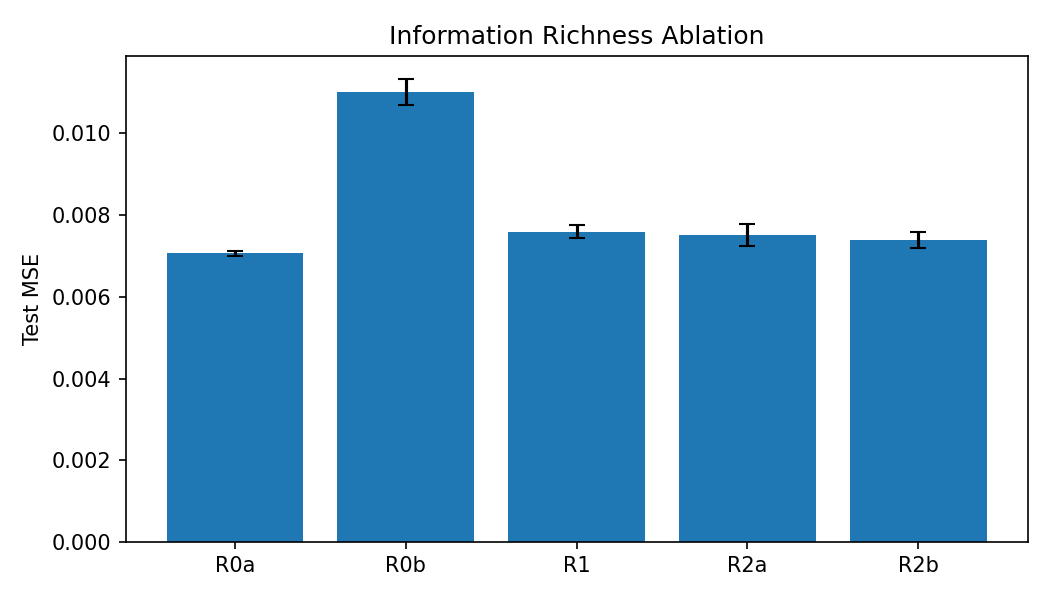
\includegraphics[width=0.95\linewidth]{phase2_mse_bar.png}
\caption{Test MSE by condition (mean $\pm$ std over 3 seeds).}
\label{fig:bar}
\end{figure}

\subsection{Pairwise Significance}

We perform paired $t$-tests over per-sample MSE values (averaged across the
three seeds) on the test set. The dominant signal is the gap between R0b and
every cross-attention condition; differences among caption-bearing conditions
(R0a, R1, R2a, R2b) are within $\sim$1 standard deviation of each other.
\textcolor{red}{[TODO: paste paired-$t$ output table from notebook cell~18.]}

\subsection{Per-Class and Architectural Effects}

The dominant classes (Tree, Grass, Crop) account for most of the MSE budget
in every condition. The rare class \emph{Shrub} is the hardest: R0b achieves
slightly negative $R^2$ on Shrub, while all cross-attention conditions reach
small positive $R^2$ values ($\approx$0.04--0.08). The Built-up class shows
the largest spread in $R^2$ across conditions (0.14 for R0b; 0.62--0.71 for
R0a/R2b), suggesting that additional fusion capacity --- not the text per
se --- helps the model separate it from Barren and Tree.

\subsection{Cross-Attention Visualization}

Fig.~\ref{fig:attn} overlays mean cross-attention weights (49 patches, mean
over 77 text tokens) on four test tiles from the R2a checkpoint at seed 42.
Attention concentrates on visually salient regions consistent with caption
topics (vegetated patches, channel boundaries) but does not, on inspection,
follow caption phrases tightly --- consistent with the non-improvement we
observe.

\begin{figure}[ht]
\centering
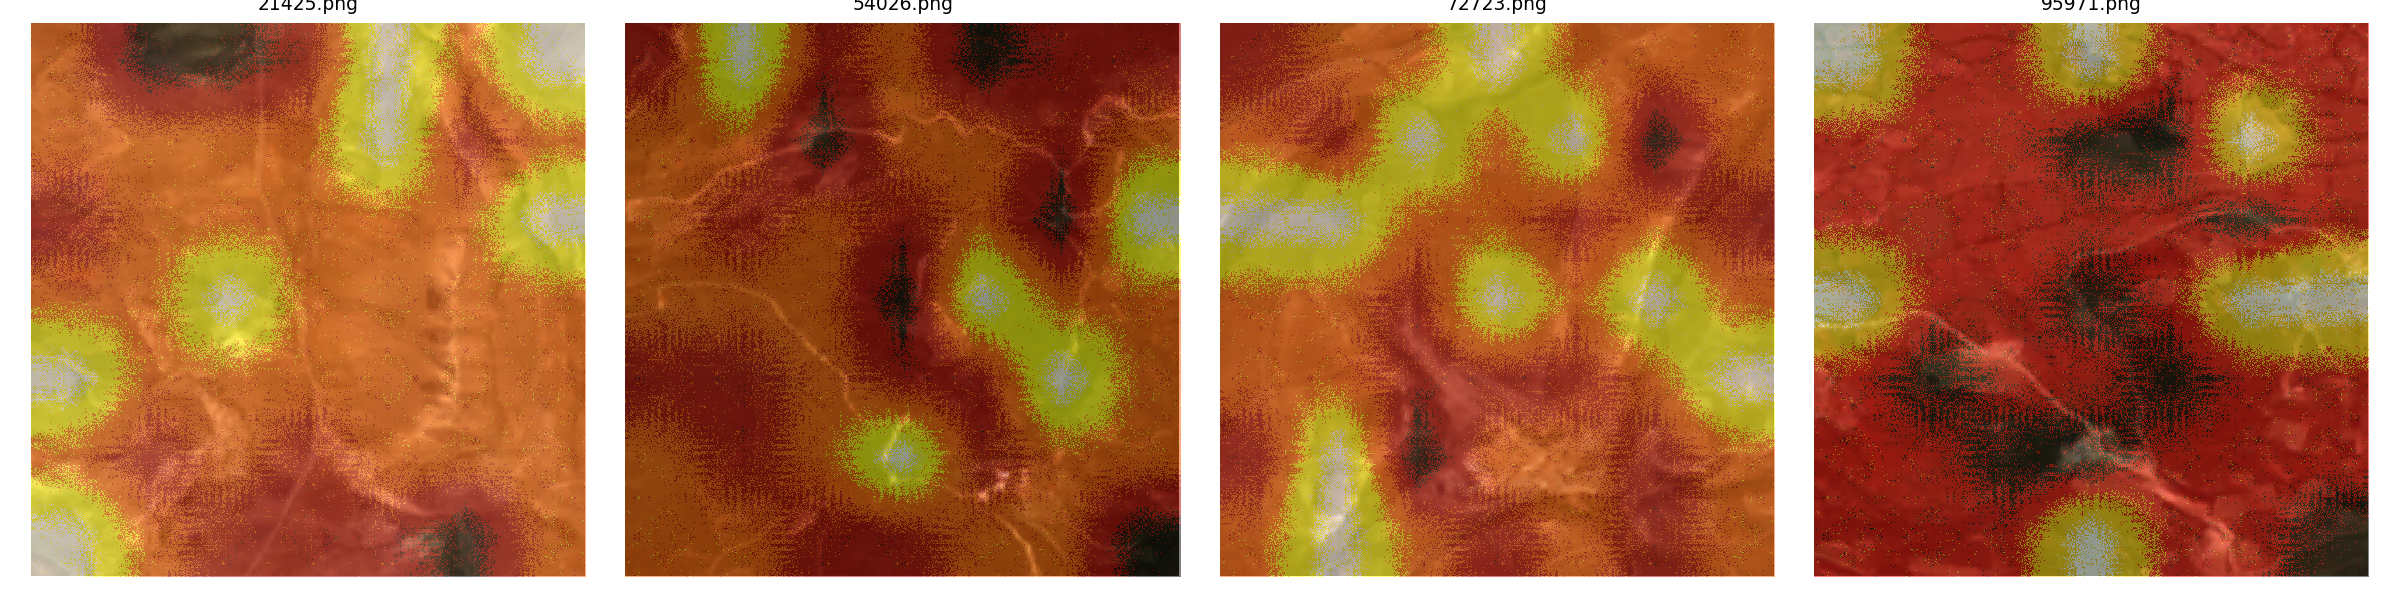
\includegraphics[width=0.95\linewidth]{phase2_attention.png}
\caption{R2a (sanitized \texttt{vision\_gemma3-4b}) cross-attention heatmaps
on four test tiles.}
\label{fig:attn}
\end{figure}

%-------------------------------------------------------------------------
\section{Discussion}

\subsection{The architectural control was load-bearing}

The single largest effect in Table~\ref{tab:mse} is the gap between R0a
(0.00707) and R0b (0.01101), a $\sim$36\,\% relative reduction in MSE
attributable not to text but to the cross-attention block being present at
all. Had we trained only R0a, R1, R2a, and R2b --- the design implied by the
original Phase 1 plan --- we would likely have credited this gain to text.
The R0b control rules that out.

\subsection{Within-fusion text yields no significant gain}

Among R0a, R1, R2a, and R2b, all means lie within roughly half a standard
deviation of each other (0.00707--0.00760). R0a, with no caption content,
is numerically the best. Two complementary explanations are plausible.

\textbf{(a) Vision captions are noisy proxies for the image.} The two
\texttt{vision\_*} models are themselves vision-language systems whose
description of a tile can be wrong: for tile \texttt{0073.png}, both models
described an arid, rocky landscape, while the ground truth is 92\,\% grass.
A model conditioned on systematically biased text may be drawn away from
the visual signal it would otherwise exploit.

\textbf{(b) Capacity, not content, drives R0a's edge.} The cross-attention
layer with an empty caption still adds learnable parameters and a non-linear
transformation over patch features; that may suffice to absorb most of the
signal that fusion architectures normally extract from text.

These readings are not mutually exclusive. In either case, the practical
takeaway is that gains attributed to ``adding captions'' must control for
both (i) extra fusion capacity and (ii) caption fidelity to the image.

\subsection{Indirect support for the leakage hypothesis}

Phase 1 hypothesized that the apparent multimodal gain from
\texttt{hybrid\_*}/\texttt{text\_qwen} captions would partly reflect the
percentages embedded in their text. Phase 2 cannot directly test this
without re-introducing the leak, but the absence of any meaningful gain from
\emph{clean} captions is consistent with the hypothesis: when the labels are
stripped from the text, the residual qualitative content does not, in this
dataset and at this scale, carry enough independent signal to improve over
the vision-only fusion control.

\subsection{Limitations}

CLIP encoders were frozen; LoRA or full fine-tuning of either encoder might
let the model extract more signal from sanitized captions. The dataset has
10\,000 tiles in a single \texttt{synth} domain; results may not transfer to
real-world tiles or to imbalanced rare-class regimes. We use a single fusion
architecture (single-layer multi-head attention with mean pooling); deeper
fusion stacks were not explored. The R1 keyword set was deliberately built
without ground-truth-aware filtering; the price is keywords that do not
always cover the dominant classes in the tile.

%-------------------------------------------------------------------------
\section{Conclusion}

We conducted a leakage-free Information Richness ablation for multimodal
land cover composition regression on ARAS400k. Including an architectural
control (R0b) was decisive: the cross-attention fusion block, even with an
empty caption, accounts for the bulk of the apparent multimodal gain on this
dataset, while clean vision-only captions of varying richness do not
significantly improve over that empty-caption baseline. We read this both
as a methodological cautionary tale --- multimodal architectures must be
ablated against architecture-matched no-text baselines --- and as indirect
evidence that the gains observed when percentage-leaking captions are used
are unlikely to be genuinely multimodal.

%-------------------------------------------------------------------------
\section*{Reproducibility}

Code, training notebooks, checkpoints, and W\&B run history are at
\url{https://github.com/OmerFarukMerey/remote-sensing-caption-composition}.
The \texttt{src/precompute.py} module materializes all CLIP outputs once;
the full 5$\times$3 grid then runs in well under one hour on an Apple
M4 MacBook Pro.

\begin{thebibliography}{1}

\bibitem{aras400k}
M. \c{C}a\u{g}lar, ``ARAS400k: Aerial Remote-sensing Annotated Scenes,''
Zenodo dataset, 2025, \url{https://zenodo.org/records/18890661}.

\bibitem{ftransunet}
J. Ma \emph{et al.}, ``FTransUNet: Multimodal Cross-Fusion for Land
Segmentation,'' \emph{IEEE TGRS}, 2024.

\end{thebibliography}

\end{document}
